\documentclass[
    11pt,
    spanish,
	a4paper
]{article}
\usepackage[utf8]{inputenc}
\usepackage[spanish]{babel}
\usepackage{graphicx}
\usepackage{authoraftertitle}
\usepackage{float}
\usepackage{caption}
\usepackage{verbatim}
\usepackage{listings}
\captionsetup[table]{labelformat=empty}

\def\doctype{Trabajo práctico}
\title{Filtros}
\author{Gonzalo Nahuel Vaca}

\begin{document}

\makeatletter
\begin{titlepage}
	\begin{center}
		\vspace*{1cm}
		
		\Huge
		\textbf{\doctype}
		\vspace{0.5cm}
    
		\LARGE
		\@title
		\vspace{0.5cm}
    
		\textbf{Procesamiento Digital de Señales (fundamentos)}
		
		\vspace{1.5cm}
		
		\textbf{\@author}

		\vspace{1.5cm}

		
\includegraphics[width=0.8\textwidth]{img/logoFIUBA.pdf}
		
		\vfill
		Maestría en Sistemas Embebidos\\
		Universidad de Buenos Aires\\
		Argentina\\
		\today
	\end{center}
\end{titlepage}
\makeatother
\newpage

\section{Resolución}

En la figura \ref{fig:filtertest} se puede observar en color rojo el espectro de la señal original.
En particular, se puede ver una meseta que corresponde a una señal que realiza un barrido en frecuencia.
En azul se puede ver la señal original en el tiempo y en verde se puede apreciar la señal luego del filtrado.

\begin{figure}[htbp]
	\centering
	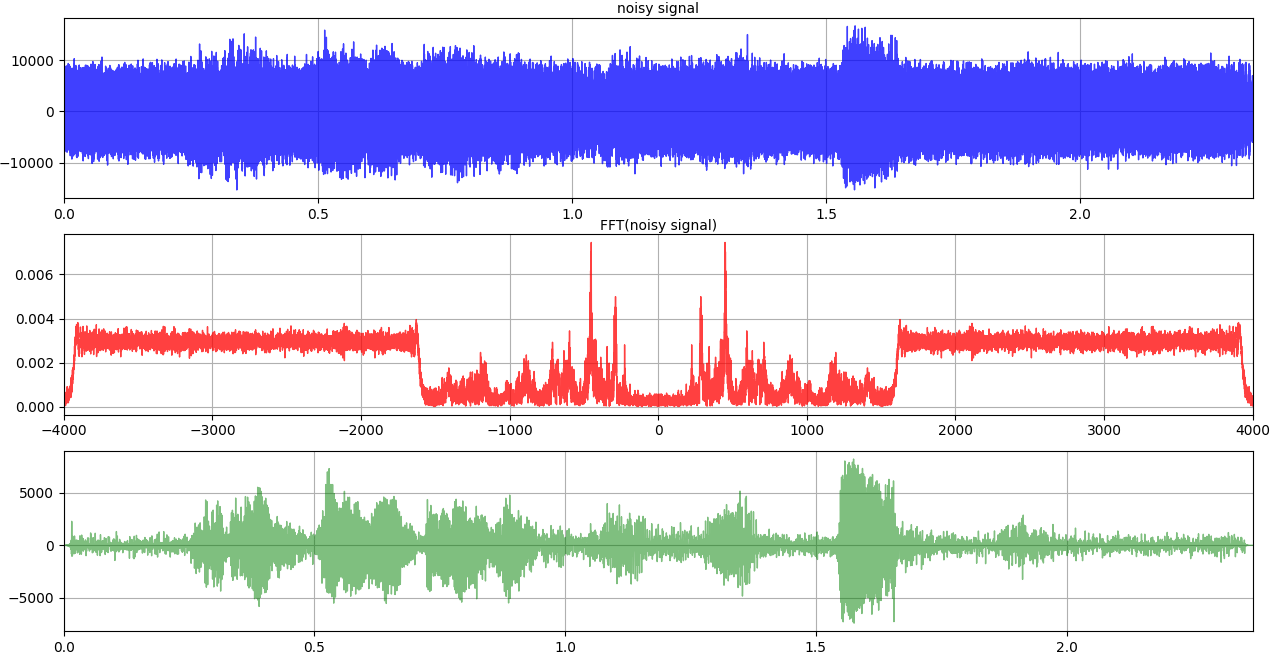
\includegraphics[width=\textwidth]{img/filterTest.png}
	\caption{Señal original y filtrada}
	\label{fig:filtertest}
\end{figure}

En la figura \ref{fig:filter} se puede observar el diseño del filtro con la herramienta pyFDA.
Se exportó el filtro y se utilizó el script provisto por la cátedra para crear un archivo fir.h
con la finalidad de usarlo en un sistema embebido.

\begin{figure}[htbp]
	\centering
	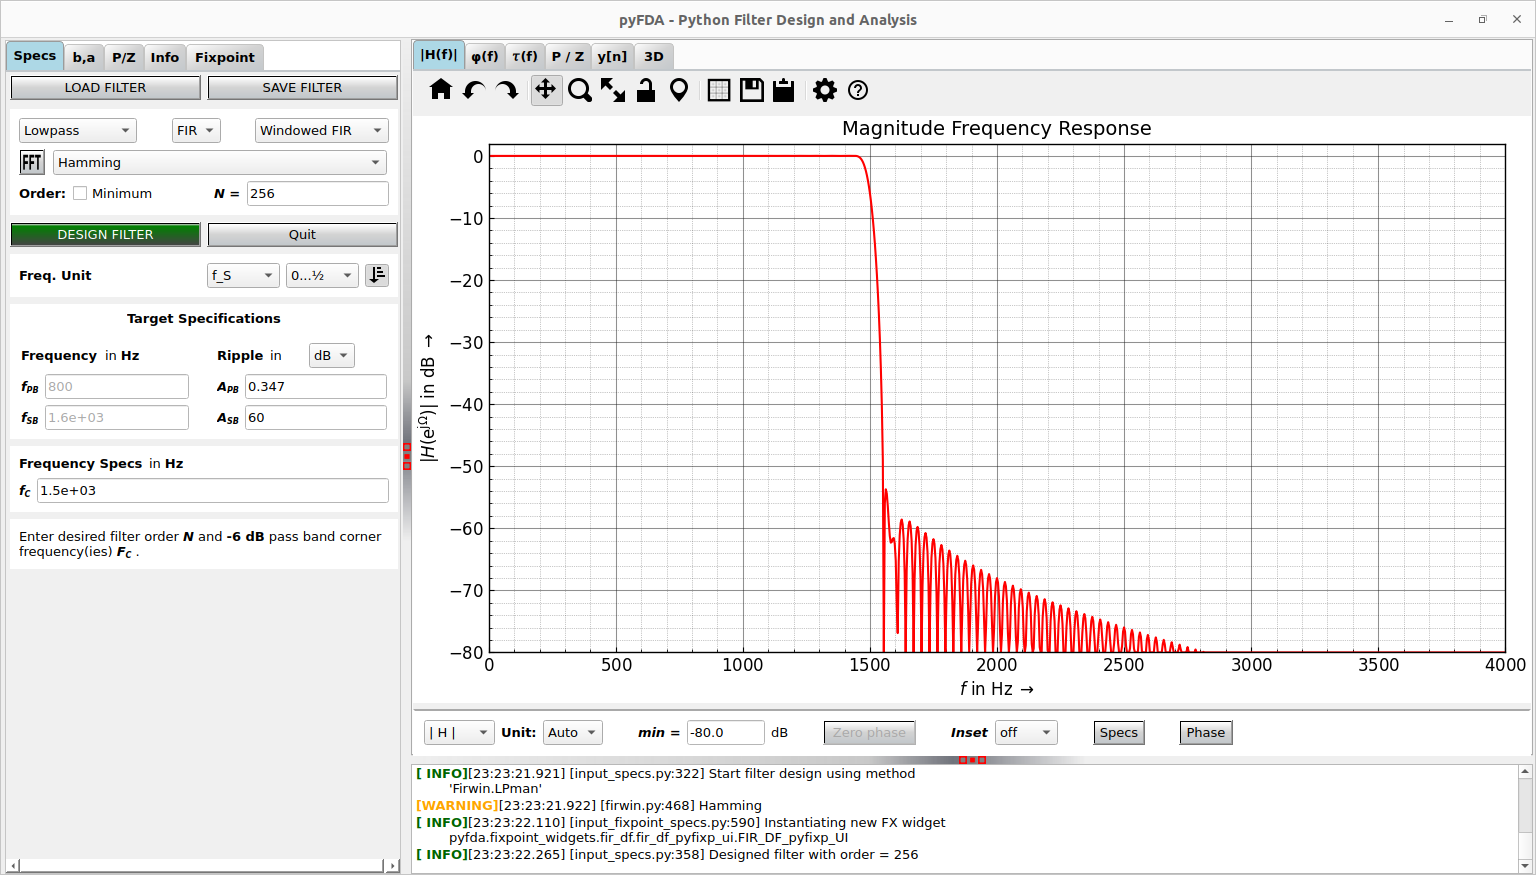
\includegraphics[width=\textwidth]{img/filter.png}
	\caption{Filtro}
	\label{fig:filter}
\end{figure}

Visualización de la señal original:

\begin{lstlisting}[
    basicstyle=\tiny,
]
import matplotlib.pyplot as plt
import numpy as np
import simpleaudio as sa


if __name__ == '__main__':
    noise = np.load('chapu_noise.npy')
    fs = 8000
    N = len(noise)
    playObj = sa.play_buffer(
        audio_data=noise, num_channels=1, bytes_per_sample=2, sample_rate=fs)

    nData = np.arange(0, N, 1)
    fData = nData * (fs / N) - (fs / 2)

    fig = plt.figure()
    noise_ax = fig.add_subplot(3, 1, 1)
    noise_ax.set_xlim(0, N / fs)
    noise_ax.set_title("noisy signal", rotation = 0, fontsize = 10, va ="center")
    plt.plot(nData / fs, noise, 'b-', linewidth = 2, alpha = 0.75)
    plt.grid()

    spectrum = np.fft.fft(noise)
    spectrum_ax = fig.add_subplot(3, 1, 2)
    spectrum_ax.set_xlim((-fs / 2) - (fs / N), (fs / 2) + (fs / N))
    spectrum_ax.set_title("FFT(noisy signal)", rotation = 0, fontsize = 10, va ="center")
    plt.plot(fData, np.abs(np.fft.fftshift(spectrum) / N ** 2), 'r-', linewidth = 2, alpha = 0.75)
    plt.grid()

    plt.show()
\end{lstlisting}

Prueba del filtro antes de realizar el código en C:


\begin{lstlisting}[
    basicstyle=\tiny,
]
import simpleaudio as sa
import numpy as np
import matplotlib.pyplot as plt


if __name__ == '__main__':

    fs = 8000
    noise = np.load('chapu_noise.npy')
    N = len(noise)

    filter_test = np.array(np.load('filter.npy')[0]).astype(float)
    filtered = np.convolve(filter_test, noise)
    playObj = sa.play_buffer(np.array(np.real(filtered), np.int16), 1, 2, fs * 1)

    N_ = len(filter_test)
    nData_ = np.arange(0, N, 1)
    fData_ = nData_ * (fs / N) - (fs / 2)

    nData = np.arange(0, N, 1)
    fData = nData * (fs / N) - (fs / 2)

    fig = plt.figure()
    noise_ax = fig.add_subplot(3, 1, 1)
    noise_ax.set_xlim(0, N / fs)
    noise_ax.set_title("noisy signal", rotation = 0, fontsize = 10, va ="center")
    plt.plot(nData / fs, noise, 'b-', linewidth = 1, alpha = 0.75)
    plt.grid()

    spectrum = np.fft.fft(noise)
    spectrum_ax = fig.add_subplot(3, 1, 2)
    spectrum_ax.set_xlim((-fs / 2) - (fs / N), (fs / 2) + (fs / N))
    spectrum_ax.set_title("FFT(noisy signal)", rotation = 0, fontsize = 10, va ="center")
    plt.plot(fData, np.abs(np.fft.fftshift(spectrum) / N ** 2), 'r-', linewidth = 1, alpha = 0.75)
    plt.grid()

    convAxe         = fig.add_subplot(3,1,3)
    convolveNData = np.arange(0, len(filtered), 1)
    convolveTData = convolveNData/fs
    convLn,       = plt.plot(convolveTData, filtered, 'g-', label ="clean signal", linewidth = 1, alpha = 0.5)

    convAxe.grid(True)
    convAxe.set_xlim(0,convolveTData[-1])

    plt.show()
\end{lstlisting}

Código C para la placa EDU-CIAA:


\begin{lstlisting}[
    basicstyle=\tiny,
]
#include "arm_const_structs.h"
#include "arm_math.h"
#include "fir.h"
#include "sapi.h"

#define BITS 10

struct header_struct
{
    char pre[8];
    uint32_t id;
    uint16_t N;
    uint16_t fs;
    uint16_t hLength;
    char pos[4];
} __attribute__((packed));

struct header_struct header = {"*header*", 0, 128, 8000, h_LENGTH, "end*"};
int16_t offset = 512;
int16_t zero = 0;

int main(void)
{
    uint16_t sample = 0;
    int16_t adc [header.N];
    int16_t y [h_LENGTH + header.N - 1];
    boardConfig();
    uartConfig(UART_USB, 460800);
    adcConfig(ADC_ENABLE);
    dacConfig(DAC_ENABLE);
    cyclesCounterInit(EDU_CIAA_NXP_CLOCK_SPEED);
    for (;;)
    {
        cyclesCounterReset();
        adc[sample] = (((int16_t)adcRead(CH1) - 512) >> (10 - BITS)) << (6 + 10 - BITS);
        dacWrite(DAC, y[sample]); // will be 128 samples delayed from input.
        if (++sample == header.N)
        {
            gpioToggle(LEDR);
            sample = 0;
            arm_conv_q15(adc, header.N, h, h_LENGTH, y);
            header.id++;
            uartWriteByteArray(
                UART_USB,
                (uint8_t *)&header,
                sizeof(struct header_struct));
            for (int i = 0; i < (header.N + h_LENGTH - 1); i++)
            {
                uartWriteByteArray(
                    UART_USB,
                    (uint8_t *)(i < header.N ? &adc[i] : &offset),
                    sizeof(adc[0]));
                uartWriteByteArray(
                    UART_USB,
                    (uint8_t *)(i < h_LENGTH ? &h[i] : &zero),
                    sizeof(h[0]));
                uartWriteByteArray(
                    UART_USB,
                    (uint8_t *)(&y[i]),
                    sizeof(y[0]));
            }
            adcRead(CH1);
        }
        gpioToggle(LED1);
        while (cyclesCounterRead() < EDU_CIAA_NXP_CLOCK_SPEED / header.fs)
            ;
    }
}
\end{lstlisting}

\end{document}